\section{EXPERIMENTS}\label{sec:expe}
To demonstrate possible effects of the system, a policy was created using parameters and variables found reasonable by the authors. These are what the insurance company would have to decide on as well. The chosen parameters and values can be seen in tables \ref{tab:roadtypevalues}, \ref{tab:crittimevalues}, \ref{tab:speedingvalues}, \ref{tab:accelerationvalues}, \ref{tab:basevalues}, and \ref{tab:polyvalues}. 

To test this policy, and thereby the developed system, trips were handpicked from the INFATI dataset. This was done on the following criteria:

\begin{itemize}
  \item Trips should follow similar routes
  \item Trips should be similar in distance
  \item Trips should display different driving styles
\end{itemize}

From these criteria, two different test cases were picked. The trips included in these cases are visualized in figures \ref{fig:shorttrips} and \ref{fig:longtrips} with two and three trips respectively. 
Test case 1, visualized in \ref{fig:shorttrips} represent two \textasciitilde8.1km equal trips, driven back and forth with the same car. The route taken is simple and has very few turns.
Test case 2 can be seen in figure \ref{fig:longtrips}. These are longer and more complex trips between  \textasciitilde31.7km and \textasciitilde32.0km. The trips involve two different cars.

For traditional insurance, the car owners would be accountable for just the distance driven. Thus, in the two test cases, the trips would cost approximately the same. With more data to look at, we can see why this should not be the case.

Looking at the data from test case 1 (\ref{tab:shorttrips}), accelerations, brakes and jerks are very similar, both in count and distribution across intervals. Green trip has slightly higher counts, but the distributions reveal no clear winner across the categories. While the trips were driven on the same route, these similarities are not a given, but can possibly be attributed to the same driver driving both trips. Speeding, however, sets these trips apart. In spite of the similarities, the car sped over triple on green trip, compared to red trip. 3.24 kilometers of speeding on an 8.08 kilometer trip is a lot, and should cost more than the 1.02 kilometers on red trip.

\begin{table}
    \begin{tabular}{lll}
    \textbf{Score type} & \textbf{Green trip} & \textbf{Red trip} \\ \hline
    Base                & 8076,23             & 8070,52           \\
    RoadType            & 355,35              & 407,56            \\
    Critical time       & 0                   & 0                 \\
    Speeding            & 2282,91             & 718,86            \\
    Acceleration        & 239,44              & 216,54            \\
    Brake               & 939,53              & 753,05            \\
    Jerk                & 213,27              & 158,06            \\ \hline
    \textbf{Total}      & \textbf{12106,72}   & \textbf{10324,60} \\ \hline
    \end{tabular}
    \caption{Trip scores for test case 1}
    \label{tab:shorttripscores}
\end{table}

\begin{table}
    \begin{tabular}{llll}
    \textbf{Score type} & \textbf{Red trip} & \textbf{Green trip} & \textbf{Purple trip} \\ \hline
    Base                & 31763,97            & 31660,97          & 32043,83             \\
    RoadType            & 873,51              & 696,54            & 720,99               \\
    Critical time       & 0                   &  237,46           & 0                    \\
    Speeding            & 12291,53            & 2544,64           & 8,96                 \\
    Acceleration        & 431,74              & 914,66            & 115,16               \\
    Brake               & 1996,90             & 1778,41           & 317,33               \\
    Jerk                & 998,09              & 2857,83           & 384,12               \\ \hline
    \textbf{Total}      & \textbf{48355,73}   & \textbf{40690,52} & \textbf{33590,39}    \\ \hline
    \end{tabular}
    \caption{Trip scores for test case 2}
    \label{tab:longtripscores}
\end{table}

\begin{table*}
    \begin{tabular}{>{\bfseries}l|ll|}
    Figure color             & Green               & Red                 \\
    Car ID                   & 16                  & 16                  \\
    Weekday                  & Thursday            & Thursday            \\
    Start                    & 18:35:59            & 19:02:22            \\
    End                      & 18:44:15            & 19:11:24            \\
    Distance (km)            & 8.08                & 8.07                \\
    Distance sped (km)       & 3.24                & 1.02                \\
    Accelerations ($>$5m/s)  & 23                  & 21                  \\
    Brakes ($>$5m/s)         & 40                  & 38                  \\
    Jerks ($>$5m/s)          & 15                  & 14                  \\
    Roadtype intervals       & 0 0 0 88 0 0 0 0    & 0 0 0 93 0 0 2 0    \\
    Speeding intervals       & 56 41 2 2 0 0 0 0   & 62 28 5 5 0 0 0 0   \\
    Acceleration intervals   & 0 0 87 0 4 9 0 0    & 0 0 67 10 24 0 0 0  \\
    Brake intervals          & 0 0 48 20 18 10 5 0 & 0 0 50 24 16 11 0 0 \\
    Jerk intervals           & 0 0 60 20 13 7 0 0  & 0 0 71 14 14 0 0 0  \\
    \end{tabular}
    \caption{Trip data for test case 1}
    \label{tab:shorttrips}
\end{table*}

\begin{table*}
    \begin{tabular}{>{\bfseries}l|lll|}
    Figure color            & Green                & Red                 & Purple             \\
    Car ID                  & 10                   & 10                  & 14                 \\
    Weekday                 & Friday               & Sunday              & Tuesday            \\
    Start                   & 22:42:35             & 18:56:50            & 08:56:15           \\
    End                     & 23:11:42             & 19:23:45            & 09:29:19           \\
    Distance (km)           & 32.04                & 31.76               & 31.67              \\
    Distance sped (km)      & 0.02                 & 13.06               & 3.63               \\
    Accelerations ($>$5m/s) & 16                   & 49                  & 34                 \\
    Brakes ($>$5m/s)        & 29                   & 71                  & 55                 \\
    Jerks ($>$5m/s)         & 21                   & 56                  & 41                 \\
    Roadtype intervals      & 49 10 00 27 5  0 2 0 & 54 0 0 29 7 0 3 0   & 5800003003000200   \\
    Speeding intervals      & 100 0 0 0 0 0 0 0    & 22 96 20 60 0 0 0 0 & 78 5 4 13 0 0 0 0  \\
    Acceleration intervals  & 0 0 94 6 0 0 0 0     & 0 0 84 6 8 2 0 0    & 0 0 68 3 6 0 3 21  \\
    Brake intervals         & 0 0 90 10 0 0 0 0    & 0 0 61 13 10 6 3 8  & 0 0 62 11 5 9 0 13 \\
    Jerk intervals          & 0 0 57 24 10 5 0 5   & 0 0 64 16 7 7 4 2   & 0 0 32 5 5 2 0 56  \\
    \end{tabular}
    \caption{Trip data for test case 2}
    \label{tab:longtrips}
\end{table*}

\begin{figure}[tb]
    \centering
    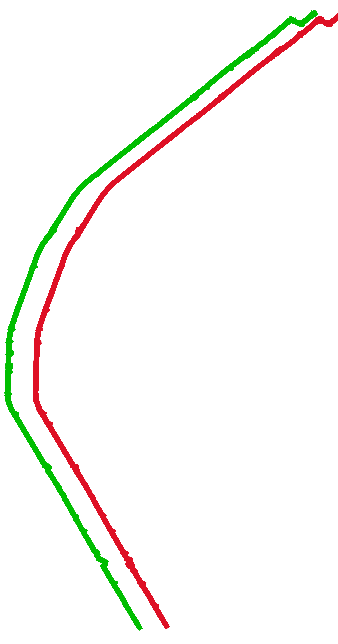
\includegraphics[width=50mm]{Pictures/ShortTrips.png}
    \caption{Short trips}
    \label{fig:shorttrips}
\end{figure}

\begin{figure}[tb]
    \centering
    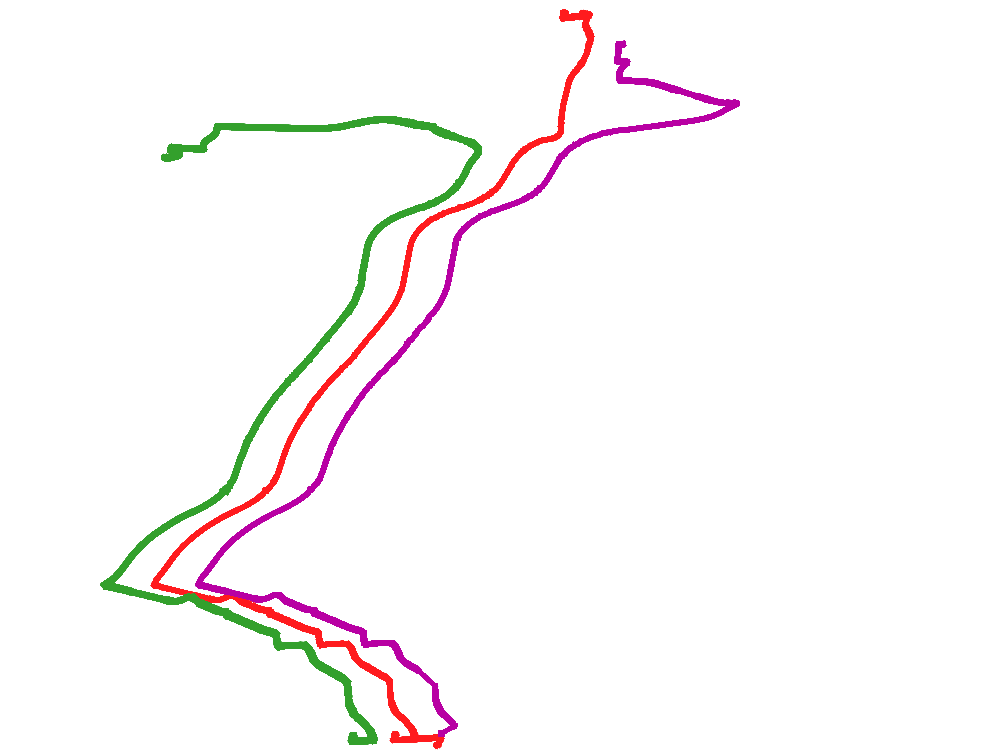
\includegraphics[width=80mm]{Pictures/LongTrips.png}
    \caption{Long trips}
    \label{fig:longtrips}
\end{figure}


\begin{table}
    \begin{tabular}{ll}
    \textbf{Roadtype} & \textbf{Weight} \\ \hline
    Motorway          & 1               \\
    Trunk             & 1               \\
    Primary           & 1               \\
    Secondary         & 1.05            \\
    Tertiary          & 1.1             \\
    Unclassified      & 1.1             \\
    Residential       & 1.2             \\
    Service           & 1.2             \\ \hline
    \end{tabular}
    \caption{Roadtypes with weights}
    \label{tab:roadtypevalues}
\end{table}

\begin{table}
    \begin{tabular}{llll}
    \textbf{Active days} & \textbf{Start} & \textbf{End} & \textbf{Weight} \\ \hline
    Monday - Friday      & 07:00:00       & 09:00:00     & 1.2             \\
    Monday - Friday      & 15:00:00       & 17:00:00     & 1.15            \\
    Saturday - Sunday    & 09:00:00       & 13:00:00     & 1.025           \\
    Saturday - Sunday    & 20:00:00       & 23:59:59     & 1.15            \\
    Saturday - Sunday    & 00:00:00       & 00:04:00     & 1.4             \\ \hline
    \end{tabular}
    \caption{Critical time intervals with weights}
    \label{tab:crittimevalues}
\end{table}

\begin{table}
    \begin{tabular}{ll}
    \textbf{Interval (\%)}   & \textbf{Weight} \\ \hline
    {[}0, 10{[}        & 1.3                   \\
    {[}10, 20{[}       & 1.4                   \\
    {[}20, 30{[}       & 1.5                   \\
    {[}30, 40{[}       & 1.6                   \\
    {[}40, 50{[}       & 1.7                   \\
    {[}50, 60{[}       & 1.8                   \\
    {[}60, 70{[}       & 1.9                   \\
    {[}70, $\infty${]} & 2                     \\ \hline
    \end{tabular}
    \caption{Speeding intervals with weights}
    \label{tab:speedingvalues}
\end{table}

\begin{table}
    \begin{tabular}{ll}
    \textbf{Interval (m/s)} & \textbf{Weight} \\ \hline
    {[}0, 3{[}              & 1               \\
    {[}3, 5{[}              & 1               \\
    {[}5, 7{[}              & 1.075           \\
    {[}7, 8{[}              & 1.1             \\
    {[}8, 9{[}              & 1.2             \\
    {[}9, 10{[}             & 1.4             \\
    {[}10, 11{[}            & 1.6             \\
    {[}11, $\infty${]}      & 1.9             \\ \hline
    \end{tabular}
    \caption{Acceleration, brake and jerk intervals with weights}
    \label{tab:accelerationvalues}
\end{table}

\begin{table}
    \begin{tabular}{ll}
    \textbf{Action} & \textbf{Base weight} \\ \hline
    Acceleration    & 50                   \\
    Brake           & 75                   \\
    Jerk            & 62.5                 \\ \hline
    \end{tabular}
    \caption{Base weights for accelerations, brakes and jerks}
    \label{tab:basevalues}
\end{table}

\begin{table}
    \begin{tabular}{ll}
    \textbf{Parameter} & \textbf{Weight} \\ \hline
    A                  & 1.02            \\
    B                  & 1.05            \\
    C                  & 0               \\
    Polynomial degree  & 1.08            \\ \hline
    \end{tabular}
    \caption{Weights for all polynomial functions}
    \label{tab:polyvalues}
\end{table}